\documentclass[11pt]{beamer}
\usepackage{hyperref}
\usepackage{booktabs}
\usepackage{xspace}
\usepackage{color,xcolor}

\begin{document}
\title{PSYC 315 Wk3 Notes}
\author{
Hsuan}

\maketitle

\begin{frame}{Table of contents}
  \setbeamertemplate{section in toc}[sections numbered]
  \tableofcontents%[hideallsubsections]
\end{frame}
\section{{\bf{\LARGE{\color{blue}Sociocultural Theories (Vygotsky)}}}}
\begin{frame}{{\bf{\LARGE{\color{violet}Intro for Sociocultural Theories}}}}
\begin{itemize}
\item Children are intertwined with other people who were eager to help them learn skills\item Cognitive development occurs in interpersonal contact\item Children are the products of their cultures\end{itemize}

{\bf{\LARGE{\color{yellow}(Emphasize cognitive development that involves symbol, artifacts, skills, and values)}}}\leavevmode\newline
\end{frame}
\begin{frame}{{\bf{\LARGE{\color{violet}Zone of proximal development}}}}
Range between what children can do unsupported and with optimal social support (social scaffolding)\leavevmode\newline
\end{frame}
\begin{frame}{{\bf{\LARGE{\color{violet}Social Scaffolding}}}}
More competent people provide temporary frameworks that lead children to higher-order thinking\leavevmode\newline
\end{frame}
\begin{frame}{{\bf{\LARGE{\color{violet}How Cognitive Change Occurs?}}}}
\begin{itemize}
\item Joint attention: process by which you focus on the same examples I am describing\item Intersubjectivity: mutual understanding established during communication - “meeting of the minds” (same understanding about something)\item Social referencing: children look to social partners for guidance about how to respond to unfamiliar events\end{itemize}

\end{frame}
\begin{frame}{Visual Cliff And Social Referencing(pic)}
There’s a clear plastic or glass floor that infants are unsure whether it is safe to cross. They look to their caregiver for cues (social referencing) as to whether it is safe or not.\leavevmode\newline
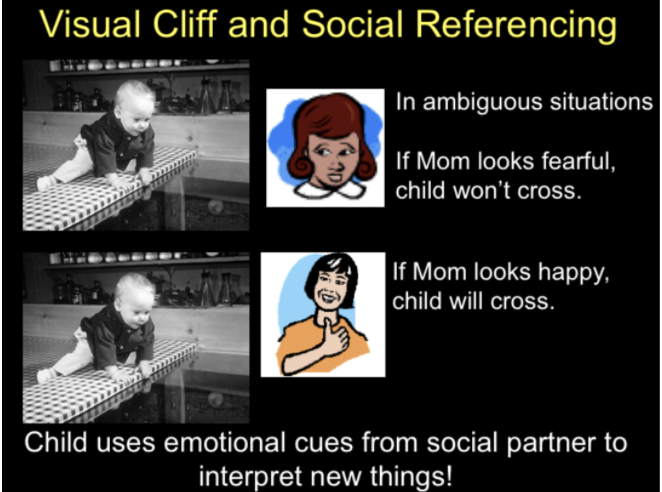
\includegraphics[width=\textwidth]{test/picForVisual.png}
\end{frame}
\section{{\bf{\LARGE{\color{blue}Ecological Theories of development: The Bioecological Model}}}}
\begin{frame}{{\bf{\LARGE{\color{cyan}Intro for The Bioecological Model}}}}
Multiple levels of environmental influence that can directly and indirectly influence a child (nested model of environmental influence)\leavevmode\newline
\end{frame}
\end{document}
